\makeatletter[H]
\renewcommand{\fnum@figure}{Figure \thefigure}
\makeatother

\chapter{Experiments and Results} \label{chap:experiments}

To show that using Dirichlet Multinomial Regression provides richer and more valuable information than single-output or deterministic methods alone, we ran experiments on the data obtained from the ACFR's Sirius AUV and Schmidt's Falkor. As seen in the previous chapter, a key benefit to applying the Dirichlet Multionomial distribution to the data is that it able to naturally perform multi-output predictions that correctly sum back to $1$ (for the normalised case). To illustrate this point, we will also compare how other methods fare when coerced to perform multiple predictions across each normalised label distribution, such as Gaussian Processes, Linear Regression, and Random Forest Regression as well, with the appropriate data projection to maximise performance. However, an important point to keep in mind is that these latter models do not intrinsically maintain the constraint of the predictions per point summing back to $1$, meaning that they are technically incorrect, but they have been included in the experiments to illustrate if they can still provide reasonable results with the advantage of having implementations more readily available in open source libraries.

We also explored how to use the data to extract information about biodiversity and the corresponding confidence, indicated by the predictive variance in the case of Gaussian Processes and Dirichlet Multinomials. Moreover, to contrast the Dirichlet Multinomial's ability to naturally provide information about co-existing habitats with certainty, we compared the regions in which the Dirichlet Multinomial with certain with the Gaussian Process, looking at both the overlapping predictions and level of variance observed in both models.

\section{Training Data}
To perform our experiments, bathymetry data and images of Scott Reef Central were used (the reef in the centre of \autoref{fig:scottreefaerial}). The bathymetry data was collected using Eric Schmidt's Falkor at the locations in \autoref{fig:gridsplit}, a ship dedicated to marine research, and the (over 700GB) of images corresponding to all the bathymetry data was collected by The University of Sydney's Australian Centre for Field Robotic's Sirius Autonomous Underwater Vehicle (AUV). The training set provided already had labels assigned, which was a result of previous efforts using Variational Dirichlet Processes that performed the unsupervised clustering \citep{steinberg11}. \todo{(currently not relevant/no context for next sentence)} On close inspection, the UTM coordinates in the training set do not correspond to the original data available from \cite{squidle} - this was because the exact point of retrieval for the bathymetry and image weren't exact matches. To account for this, labels corresponding to bathymetry points were in fact taken from the closest images, rather than exact longitude/latitude or UTM matches, although the UTM coordinates in the training data itself remains as the original. \todo{(describe the specific features - depth, aspect, rugosity, etc.)}

\begin{figure}
    \includegraphics{scott_reef_aerial.jpg}
    \caption{Aerial shot of Scott Reef from \cite{NASA:SRI}}
    \label{fig:scottreefaerial}
\end{figure}

\section{Data Preprocessing}

\subsection{Downsampling the Data}
As the purpose of using Dirichlet Multinomial Regression was to be able to model the distribution of habitat label occurrences over an area, we downsampled the combined 2011, 2015 dataset which was at a significantly higher resolution than the 2009 dataset \todo{(calculate how much perhaps)}. To do this, `grid' of squares was essentially mapped onto original space, and points in each grid grouped together into a single point. For the multi-output labels, all label counts in each lower-resolution grid were summed, whereas for the single label case, the label was selected randomly \textit{but} with more weighting to the non-sand labels, to slightly increase the variance of labels observed. The reason for doing this was because of the dominance of the 'sand` habitat - random selection when only one absolute label per point was present resulted in an even larger portion of sand than in the original dataset, causing predictions on the full query data to sometimes result in almost $100\%$ sand, even moreso than was already the case in \autoref{fig:det4maps}.

% Two methods of downsampling in particular were tested. The first coarser approach involved simply taking the space in which the data was collected and placing grids of fixed size over them as in \cref{fig:gridsplit}, binning all points falling within each grid into a single datapoint. Each of these data points contained multiple points from the original dataset with their own counts for each of the possible labels, so the downsampled points simply took the sum of all the label counts in each fixed grid. 
% 
% The second summed label counts in the same way, but clusters were instead formed by first calculating the full dendrogram on the 16502 entries in the training data, and forming groups such that none had more than 5 of the original points within them, and the sub-clusters (at each level of the dendrogram) were no more than a 21 metres away from one another. As can be seen in \cref{fig:dendrogram}, the gradual merging into the single supercluster was quite consistent, indicating the original datapoints were mostly evenly distributed.
% 
% \todo{(cut down this section (probably down to one paragraph) - and also talk about how for the single label case, instead of summing counts for the new 'label', labels were chosen at random (for more variance in the GP which is otherwise too certain about everything being sand))}
% 
\begin{figure}[H]
    \includegraphics[scale=0.6]{training_map_fixedgrid.pdf}
    \caption{Fixed-sized grids placed over training data \todo{(redo this plot nicely!)}}
    \label{fig:gridsplit}
\end{figure} 
% \begin{figure}[H]
%     \centering
%     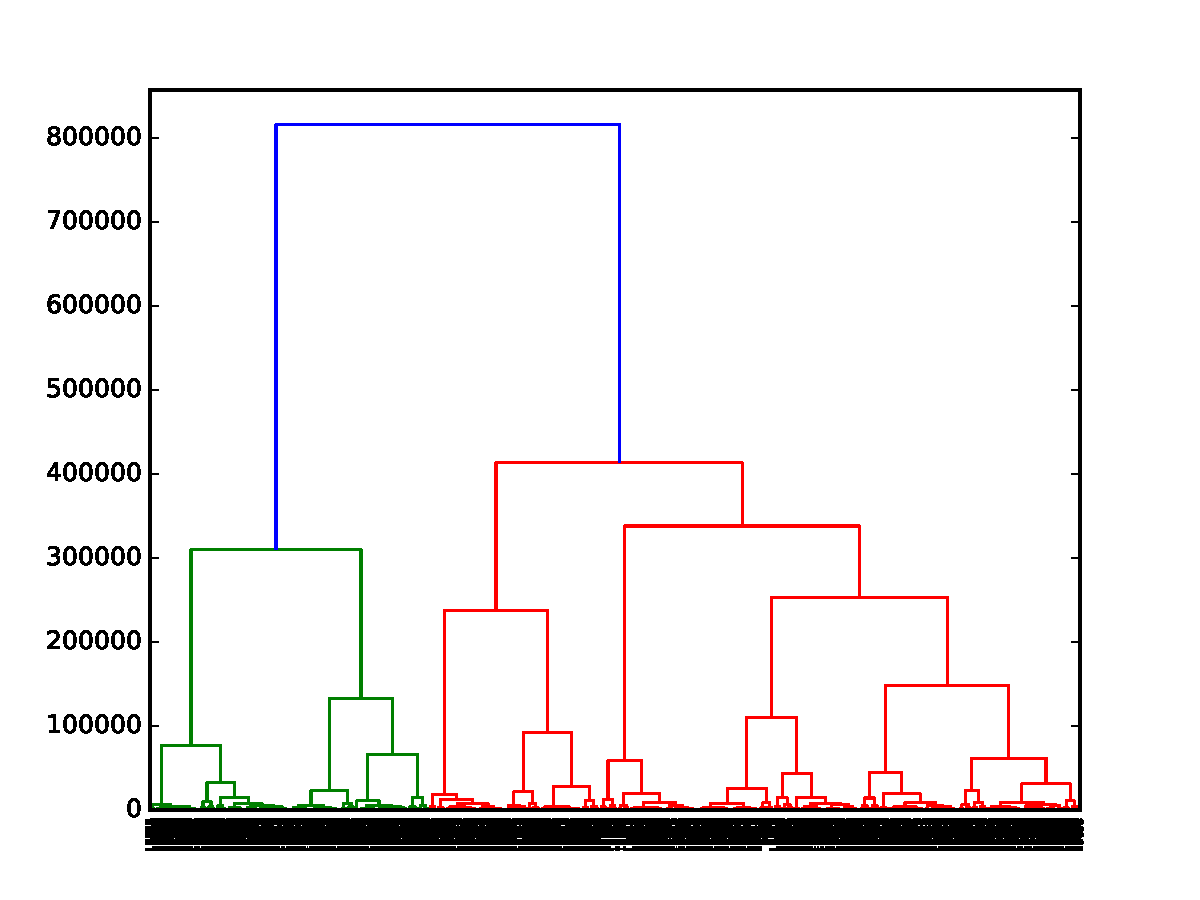
\includegraphics[scale=0.6]{dendrogram.pdf}
%     \caption{Dendrogram of training data}
%     \label{fig:dendrogram}
% \end{figure}

\subsection{Simplifying labels}
Another preprocessing step that was performed was the aggregation of habitat labels. The original training data contained 24 separate labels determined through an automated clustering procedure using Dirichlet Processes. Because of the uneven distribution of these labels (\autoref{fig:singlelabeldistr} and \autoref{fig:multilabeldistr}), with the occurrence of some too insignificant for any machine learning algorithms to pick up, they were simplified in collaboration with ecological experts, who manually identified which of the 24 labels were in fact of the same class - for example, 5 separate classes of coral may have been indistinguishable to the average person, and were hence grouped into a single label. This allowed the near-non-occurring labels to be grouped together with more commonly occurring ones, whilst also allowing a different level of granularity in training models/forming predictions that could be used if only an approximation equivalent to observable human differences of an area's benthic map were required. Moreover, due to the unsupervised nature of the labeling, certain clusters were notably \textit{inconsistent} with the rest, for example when sea cucumbers became the identifying feature of one of the 24 labels.

\begin{table}[H]
    \centering
    \begin{tabular}{|c| c|}
        \hline
        simplified & original \\\hline
        0 & 1, 2, 18, 20, 21, 23, 24 \\
        1 & 3, 5, 10, 16, 17, 19, 22\\
        2 & 13, 14, 15 \\
        3 - Sand & 4, 6, 7, 8, 9, 11, 12 \\
        \hline
    \end{tabular}
    \caption{Full-simplified label mappings \tiny{\todo{label mappings - sand, coral, patchy coral, (?) halameda, rhodliths}}}
    \label{table:labelmappings}
\end{table}

\begin{figure}
    \includegraphics[scale=0.17]{class_mosaic_24_classes.jpg}
    \caption{Samples of images from each of the full 24 classes}
    \label{fig:24classes}
\end{figure}

\begin{figure}[H]
    \begin{minipage}{.47\linewidth}
        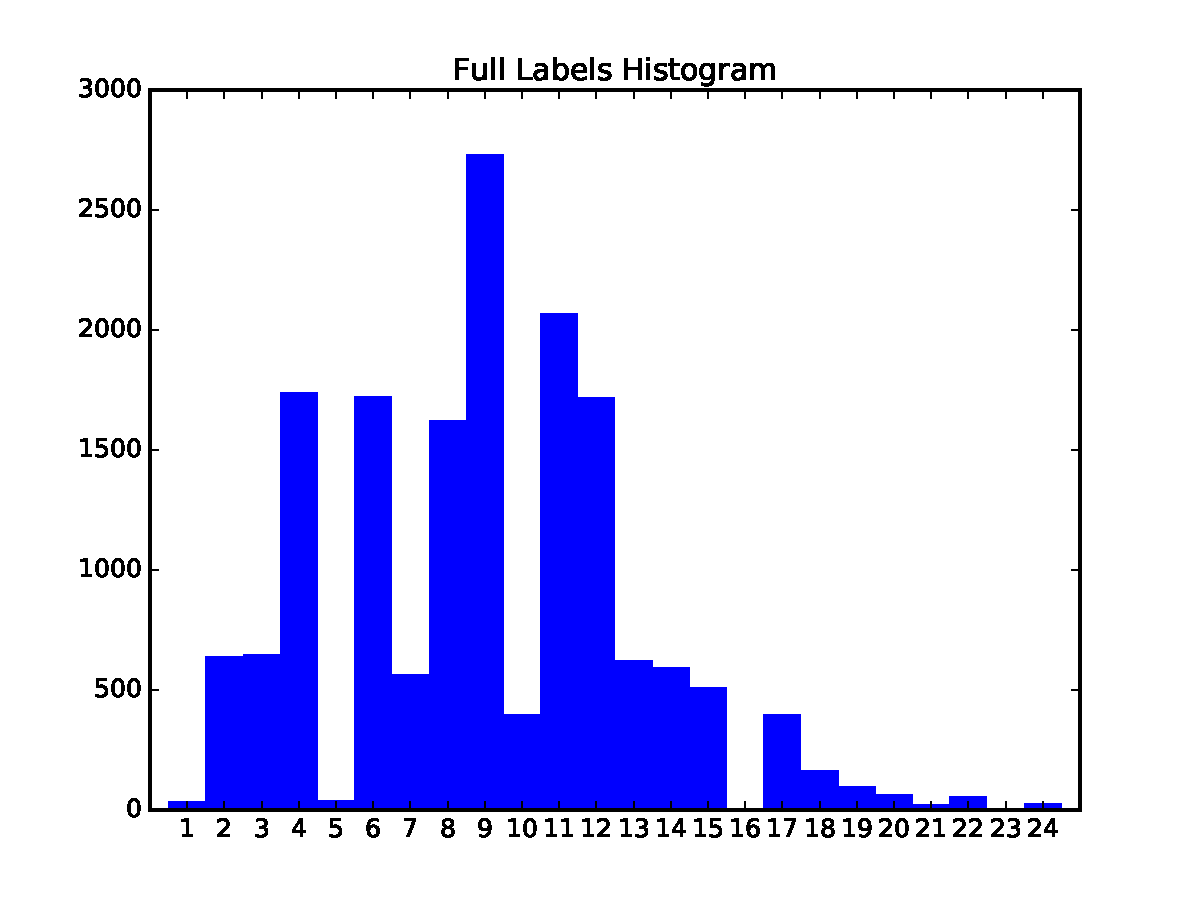
\includegraphics[width=\linewidth]{hist_full_labels.pdf}
        \caption{Distribution of labels in original dataset}
        \label{fig:singlelabeldistr}
    \end{minipage}
    \hfill
    \begin{minipage}{.47\linewidth}
        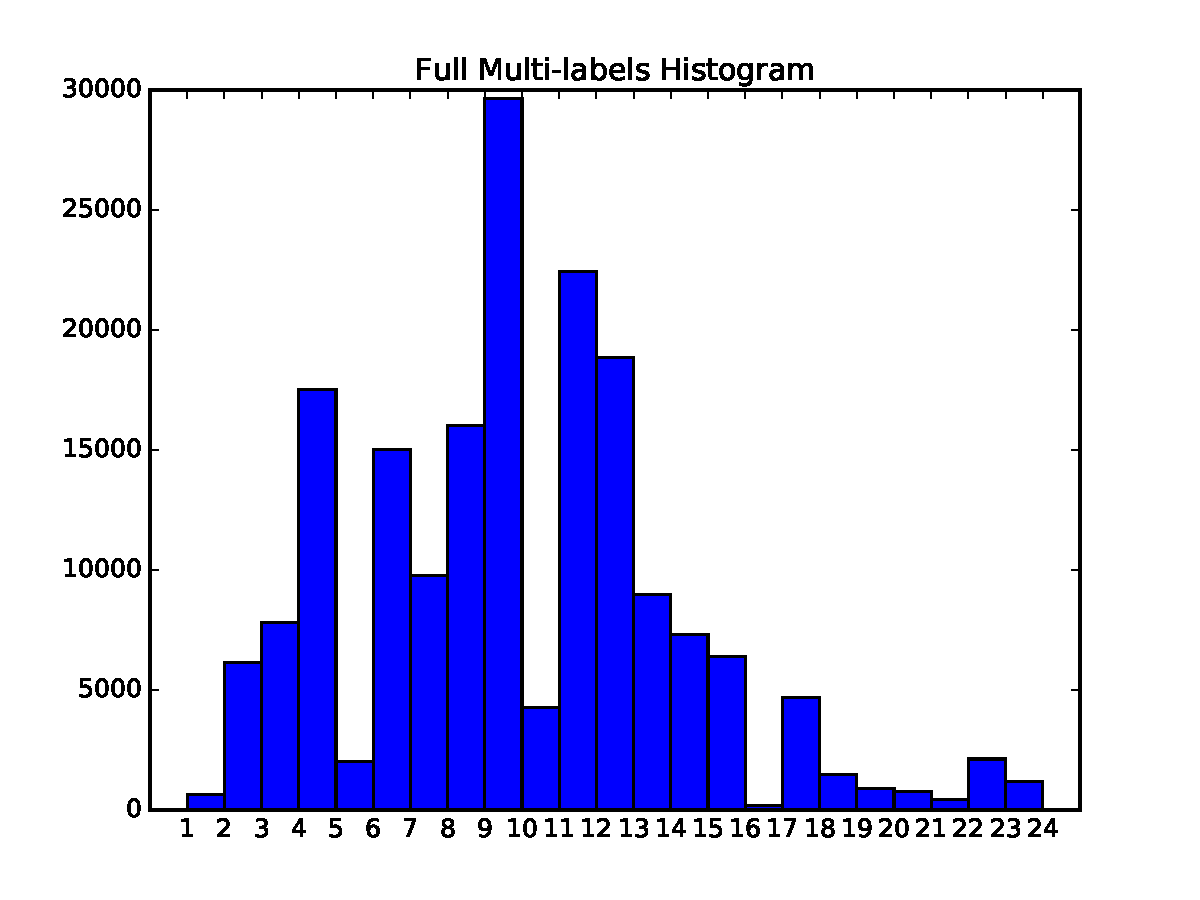
\includegraphics[width=\linewidth]{hist_full_multi_labels.pdf}
        \caption{Distribution of labels in multi-label outputs}
        \label{fig:multilabeldistr}
    \end{minipage}
\end{figure}

\begin{figure}[H]
    \begin{minipage}{.47\linewidth}
        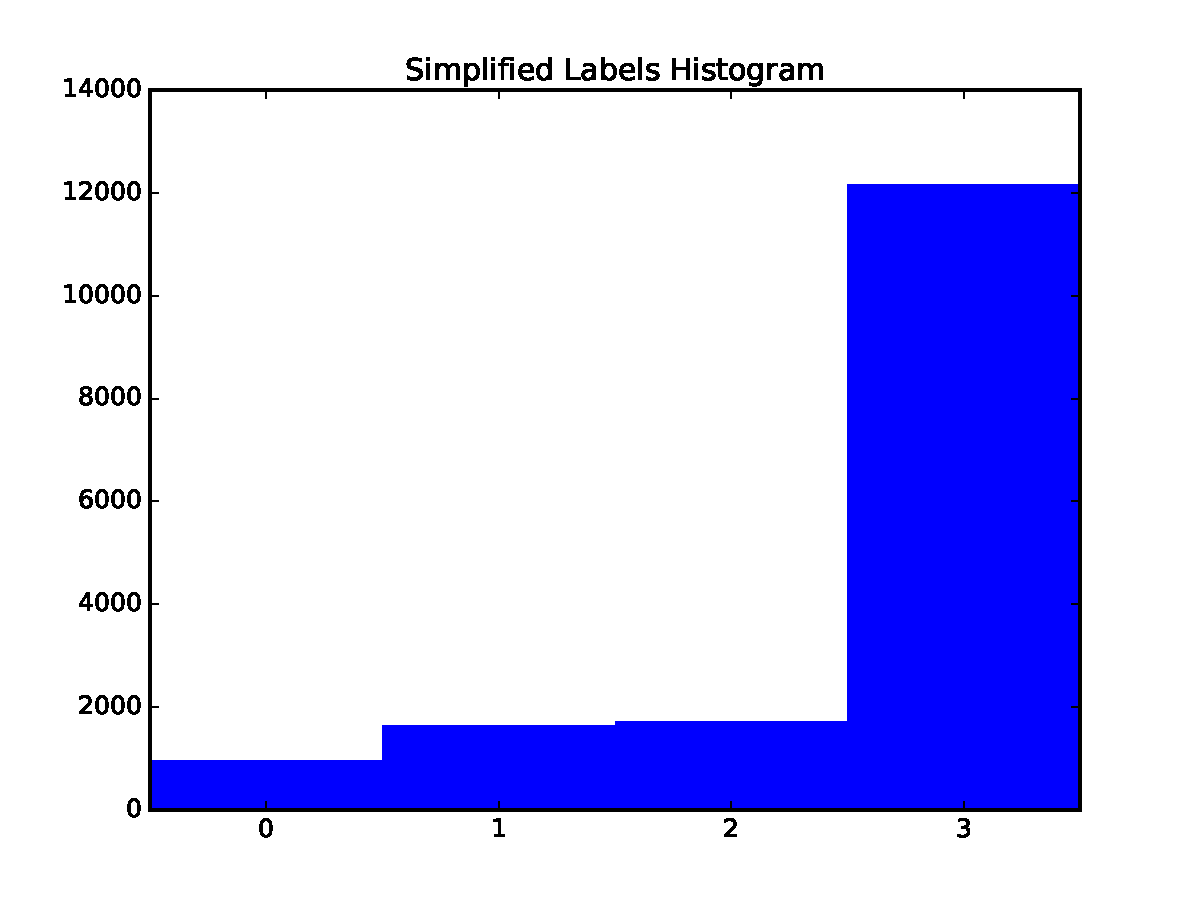
\includegraphics[width=\linewidth]{hist_simple_labels.pdf}
        \caption{Distribution of simplified labels in original dataset}
        \label{fig:singlelabeldistr}
    \end{minipage}
    \hfill
    \begin{minipage}{.47\linewidth}
        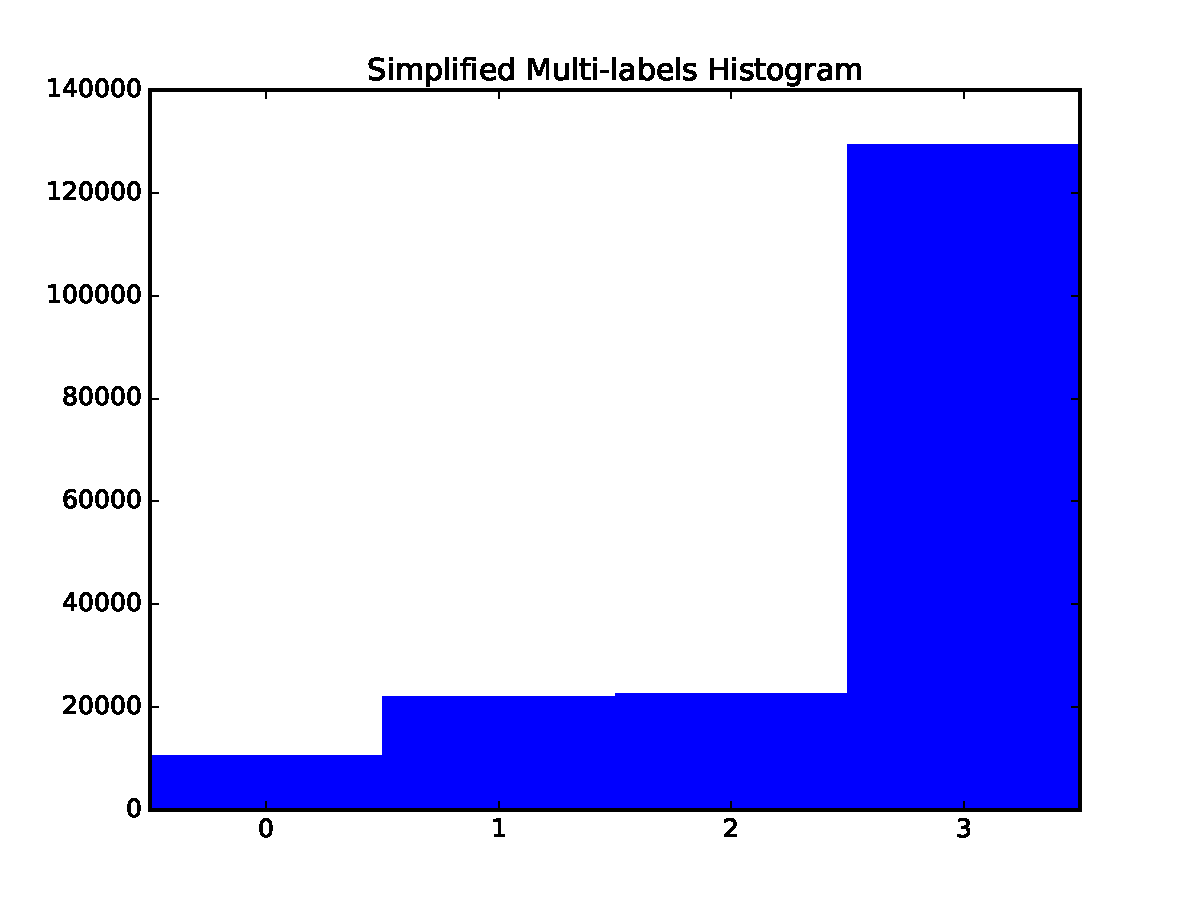
\includegraphics[width=\linewidth]{hist_simple_multi_labels.pdf}
        \caption{Distribution of simplified labels in multi-label outputs}
        \label{fig:multilabeldistr}
    \end{minipage}
\end{figure}

Note that from this point onwards, we will be working with the reduced feature set, in line with the aim of the paper to show the advantages of dirichlet multinomial regression when studies (environmental or otherwise) are limited to lower resolution data where strictly assigning only a single label to the features at a given data point is not representative of the otherwise rich information available. This restriction is a realistic one, because to be able to monitor large portions of the ocean for conservational and management reasons amongst others, data needs to be collected economically en-masse - and this means not collecting very high resolution data that would attract obscene costs at scale.

\subsection{Coordinates as features}
Due to the abundant bathymetry data that was available in the form of depth, rugosity and aspect at each available data point, there was reason not to include the coordinates themselves in the feature space. Whilst it is logical that in a natural environment, areas that were spatially close would also have similar properties, this should not be relied upon, and other intrinsic properties should be the basis upon which predictions are made. Forming predictions on the full query dataset using a random forest supports this notion quite strongly - whilst 10-fold cross validation using the coordinates as features had a notably higher F-score of 0.61 compared to 0.40 without, the unnaturally straight split between the left and right segments (\autoref{fig:rf_w_coords_preds}) over a 12km region suggests that the predictive map is flawed. Moreover, by including the coordinates as a training feature, an assertion is made about the direct relationship between a benthic location and the habitat class/es it contains, despite its other physical properties such as depth, aspect, etc. 

\begin{figure}[H]
    \begin{minipage}{.49\linewidth}
        \includegraphics[width=\linewidth]{full_predictions_randomforest.pdf}
        \caption{Full predictive map using Random Forests including coordinates as features}
        \label{fig:rf_w_coords_preds}
    \end{minipage}
    \hfill
    \begin{minipage}{.49\linewidth}
        \includegraphics[width=\linewidth]{full_predictions_randomforest_nocoords.pdf}
        \caption{Full predictive map using Random Forests excluding coordinates as features}
        \label{fig:rf_wo_coords_preds}
    \end{minipage}
\end{figure}

\subsection{Preprocessing and Feature Projection}
To maximise performance of the algorithms used across the experiments, a number of preprocessing steps were taken to improve the predictions made. The features in the data were first scaled, where each feature was centred to the mean with unit variance), then normalised over each future such that they had unit length \todo{(include plots of the diff approaches across DM/GP/others, ref plots)}. To allow the algorithms tested to learn the data and its complexities better, projecting the data into higher dimensional space was required. Full quadratic projections ($x_0, x_1, x_2 \Rightarrow x_0^2 ,x_1^2 ,x_2 ,2x_0x_1 ,2x_0x_2 ,2x_1x_2$) and squared terms with a $1$ bias terms ($x_0, x_1, x_2 \Rightarrow x_0 + x_1 , x_2 ,x_0^2 ,x_1^2, x_2^2, 1$) were both tested. The latter was chosen, one of the reasons being that it resulted in an lower average error when performing 10-fold cross-validation using Dirichlet Multinomial Regression (\autoref{table:dmbasicresults}). It was also chosen to allow predictions to run faster, and for the Markov Chain Monte Carlo for Dirichlet Multinomial Regression later in this chapter, \textbf{significantly} reduce the number of dimensions that need to be traversed - considering the number of weights required is features $\times$ number of labels, this would correspond to the 4-label data needing $19*4=76$ vs $55*4=220$ weights, and the full 24-label case requiring $19*24=456$ vs $55*24=1320$ weights.

\todo{(ref plots)}

\todo{(show plots)}

% The results from the Experiments detailed in Chapter 4 are listed below. The range of possible class values in some cases have been stretched beyond the existing class labels so that values align between different outputs to allow for easy, direct visual comparison \todo{(this hasn't actually happened yet)}. Note that the results to the above experiments will include those of both non-downsampled and downsampled results, as well as the full set of 24 labels as well as simplified ones.
% 
% Due to the low occurrence of some labels in the original dataset though, they have ended up being ommitted in predictions - these are excluded from the colour schemes of the benthic maps generated, so that those that do occur can be given more distinct colours from one another as to better differentiate between the habitats of a map, as well as allow a consistent comparison of across different maps. \todo{(again, hasn't happened yet)}

% The associated generated maps from the experiments are also provided here, but proper evaluation of them, such as what habitat clusters and relationships can be gleaned, will be explored in Chapter 5. 

\section{Single-Output Predictions}

\subsection{Deterministic Approaches}

We first briefly review the machine learning techniques more commonly used in benthic habitat mapping first, to get an idea for the sort of maps generated as well as their performance for the given dataset. To quantifiably compare their predictions, we calculate their unweighted f-scores. The \textit{f-score} of predictions are a measure of accuracy in classification problems that takes into account both precision and recall across each possible label, and is calculated by $2*\frac{\text{precision*recall}}{precision+recall}$. The use of unweighted f-scores means, we calculated the \textit{f-score} separately for each label in the predictions, and simply took the average of them. This was chosen in favour of weighted f-scores that provide a larger weight for more frequent labels as the high occurrence of sand would hide the fact that the other labels are constantly incorrectly predicted, if this was the case. Logistic regression has been included here despite containing 'probabilistic` predictions in the form of regression values passed through the \textit{logit}, and as such the results displayed are a result of simply taking the argmax over possible the predictive probability over possible for each datapoint. Those probabilistic outputs are useful for comparisons with those of Gaussian Processes, however, which will be explored in the next section. \todo{(this GP-LR comparison hasn't happened yet)}

\begin{table}
    \centering
\begin{tabular}{|c|c|c|c|c|c|}
    \hline
    Algorithm & 10F-CV F-score & 10F-CV Accuracy & Label type\\\hline
    SVC & 0.21514 & 0.75554 & 4 labels \\
    LogisticRegression & 0.33713 & 0.77001 & 4 labels \\
    KNeighborsClassifier & 0.4714 & 0.7796 & 4 labels \\
    RandomForestClassifier & 0.4737 & 0.79406 & 4 labels \\
    SVC & 0.10355 & 0.29408 & 24 labels \\
    LogisticRegression & 0.13335 & 0.31389 & 24 labels \\
    KNeighborsClassifier & 0.22593 & 0.33093 & 24 labels \\
    RandomForestClassifier & 0.22015 & 0.3405 & 24 labels \\
    \hline
\end{tabular}
\label{table:detresults}
    \caption{Performance of common machine learning models}
\end{table}

\begin{figure}[H]
    \includegraphics[width=\linewidth]{det_preds.pdf}
    \caption{Full predictive map using SVMs, Logistic Regression, kNN, and Random Forests}
    \label{fig:det4maps}
\end{figure}

While the accuracy of the Logistic Regressor, kNN, and Random Forest Classifier are reasonable (above $0.75$), the former two's f1-scores are very poor at $0.33$, with the latter two at just below $0.5$, which is an equally undesirable result. Looking at the ratio of available labels in the downsampled data in the 4-label case ($232,  470,  446, 3548$ for labels 0, 1, 2, 3 respectively) reveals that label 3 accounts for $0.7556$ of the dataset - a value very close to the accuracy of predict. The weighted f1-score of a `naive' classifier that always predicts label 3 has an accuracy of  $0.75554$ and an average f-score of $0.215$ - highlighting the fact that these simpler models are not able to produce results that confidently outperform simply guessing one label for any given datapoint. \autoref{fig:det4maps} visualises the predictions from \autoref{table:detresults} on the full query data for the 4 and 24-label data respectively\todo{(only showing 4-label(?) case atm! and need to include discrete label colourbar!)}. The Support Vector Machines (SVM) that generally provides moderately respectable real-world performance has noticably failed to predict anything other than sand throughout the query space, hinting the underlying data has complexities that require more complex models to explain it. The predictive maps generate using Logistic Regression and kNN bear noticable similarities in many areas of the map, while Random Forests identified regions that the others didn't.

\subsection{Probabilistic Approaches}
\subsubsection{Single-Output Gaussian Process Classification}
\todo{show more stratified results (not just even split) to show that even splits did better}

\begin{tabular}{|c|c|c|c|c|c|c|c|}
    \hline
    No. points & Type of split & Type of GP & Number of runs & AUROC & Notes & F1-score \\\hline
    500     & Even       & GP     &  10        & 0.86534    &                     &         \\
    500     & Stratified & GP     &  10        & 0.80136    &                     &         \\
    1000    & Even       & GP     &  1         & 0.87626    & Deterministic       & 0.56208 \\
    1000    & Even       & PoEGP  &  5         & 0.80973    &                     & 0.47481 \\
    1000    & Even       & PoEGP  &  200       & 0.80186    &                     & 0.47595 \\
    1000    & Even       & GPoEGP &  5         & 0.80864    &                     & 0.51018 \\
    1000    & Even       & GPoEGP &  200       & 0.80105    &                     & 0.47748 \\
    1000    & Even       & BCM    &  5         & 0.80682    &                     & 0.48167 \\
    1000    & Even       & BCM    &  200       & 0.80421    &                     & 0.48227 \\
    1000    & Even       & GPy    &  1         & 0.87638    & RBF, EP (default)   & 0.57013 \\
    \hline
\end{tabular}
\todo{(look at AUROC/AUC and log probabilities as well)}

\todo{highlight areas with low/high certainty, etc. NOTE - investigate the areas with visually even splits of two labels - e.g. right-side arms of label 1,2, and smaller patches in the bottom left corner of label 0,3 - show that uncertainty about whether those areas are label 1 or 2, 0 or 3 respectively, is (should) be high, and that taking argmax for the sake of visual representation within a single image hides this information}

\todo{(maps of 4-label full predictions)}

\todo{(maps of all-label full predictions)}

\section{Multi-Output Predictions} 
Looking at the maps from \autoref{fig:det4maps}, it is obvious, visually, where clusters of certain habitats are - but what can't be easily obtained, or at least automated without non-trivial extra effort, is identifying exactly \textit{where} these clusters are the frequency of co-occurrence with other nearby labels. This is a consequence of only having a single label per point, but considering the considerable area covered by a single data point, it is unrealistic to imagine the entire surface being only a \textit{single} label. Thus, we explore how to predict the \textbf{distribution} of labels at each point as represented in the original data, to provide richer habitat maps that naturally illustrate the co-occurrence of different habitats.

\subsection{Coercion of Common Regression Machine Learning Algorithms} \label{ss:commonMLcoercion}
To do this, we first look at the regression version of algorithms used in the previous section, instead applied individually to each of the label distribution values in the original dataset, rather than simplifying them down to a single habitat label. In particular, Linear Regression, Random Forest Regression, and K-Nearest Neighbour Regression were used. SVM Regression was ommitted largely due to its very poor performance in the single-label case, but also in part from the extensive computational time that would be required across predictions per label.

\begin{figure}[h]
    \title{\large{\textbf{Linear Regression}}}
    \centerline{\includegraphics{multi4_preds_lr.pdf}}
    \caption{Map of full query Linear Regression 4-label predictions}
    \label{fig:multi4_lr}
\end{figure}

\begin{figure}[h]
    \title{\large{\textbf{K Nearest Neighbour Regression}}}
    \centerline{\includegraphics{multi4_preds_kn.pdf}}
    \caption{Map of full query K Nearest Neighbour Regression 4-label predictions}
    \label{fig:multi4_rf}
\end{figure}

\begin{figure}[h]
    \title{\large{\textbf{Random Forest Regression}}}
    \centerline{\includegraphics{multi4_preds_rf.pdf}}
    \caption{Map of full query Random Forest Regression 4-label predictions}
    \label{fig:multi4_rf}
\end{figure}

As a result, demonstrating how to use multiple, independent regressors for this purpose is more an illustrative exercise than a practical one that can be relied on in the field - because the constraint that the normalised distributions should sum to $1$ at each point is violated, where in some cases \textit{no} labels exist at points, while in others, the distributions sum to as high as $3$.

\subsection{Coersion of Gaussian Process Regression}
Although a Gaussian Process is only designed to deal with single outputs, each of the label distributions per datapoint are seperate values, meaning it is possible to use multiple Gaussian Processes to allow it to work as a multi-output model. 

Average error was $0.14409166865082482$ in 10-fold CV \todo{(format)}

While the ability of a Gaussian Process allows the data to `speak for itself' aided in bringing the average sum of distributions per point to $1$ compared to the simpler models in \ref{ss:commonMLcoercion}, this property is still not inherently there, not to mention that the full query dataset of just under $3,000,000$ points was too computational intensive to perform full predictions on.

\subsection{Dirichlet Multinomial Regression}

% \begin{tabular}{|c|c|c|c|c|c|}
%     \hline
%     Algorithm & 10F-CV F1 & 10F-CV Accuracy & Parameters & Data \\\hline
%          DM         &  0.13802716811804644 & 0.37856057852908254 &            &  full labels  \\
%          DM         &   0.287405310254214  &  0.757925654489819  &            & simple labels \\ %     \hline
% \end{tabular}

\subsubsection{Parameter Selection}

To select an optimal set of parameters for the dirichlet multinomial, Markov Chain Monte Carlo (MCMC) was used to draw samples from the posterior distribution \todo{(refer to equation?)} over $3,000,000$ runs, with the maximum a posteriori estimate used as the starting value for the weights. To select the single best set of weights from the sequence of chains, every single one was evaluated by being used to do Dirichlet Multinomial regression, where the weights that resulted in the lowest predictive variance (average over all variances) was considered to be the best set of parameters. The weights that corresponded to the lowest average variance also corresponded to the lowest average error compared to the original normalised weights. After the $3,000,000$ runs, the MCMC in both cases (the simplified 24 labels, as well as the full set) was considered to have converged, as the Gelman and Rubin ($\hat{r}$) convergence statistics were calculated to be \todo{(? and ?)}, both very close to the ideal value of $1.0$, Furthermore, for the \todo{24-label case}

% MCMC 2 million runs, 24 labels
% 18-smallest variance corresponds to the 1-smallest error - index 1444288 \\
% 19-smallest variance corresponds to the 2-smallest error - index 1444289 \\
% 20-smallest variance corresponds to the 4-smallest error - index 1444292 \\
% 21-smallest variance corresponds to the 0-smallest error - index 1444291 \\
% 22-smallest variance corresponds to the 3-smallest error - index 1444290 \\

% np.save('data/W_2m_1444288', chains[1444288])
% np.save('data/W_2m_1444289', chains[1444289])
% np.save('data/W_2m_1444292', chains[1444292])
% np.save('data/W_2m_1444291', chains[1444291])
% np.save('data/W_2m_1444290', chains[1444290])

\begin{figure}[H]
    \centerline{\includegraphics{dm4_9m_0_mcmc_weight_hist.pdf}}
    \caption{MCMC weights for 4-label, 19-dimension data case \todo{(need to separate this into separate images, possibly remove axis ticks)}}
    \label{fig:4l-mcmc_weights}
\end{figure}

\begin{figure}[H]
    \centerline{\includegraphics{dm24_950k_0_mcmc_weight_hist.pdf}}
    \caption{MCMC weights for 4-label, 19-dimension data case \todo{(need to separate this into separate images, possibly remove axis ticks)}}
    \label{fig:24l-mcmc_weights}
\end{figure}

\begin{table}[H]
    \centering
    \title{Dirichlet Multinomial Regression Average Errors}
    \begin{tabular}{|c|c|}
        \hline
        Features & Root Mean Squared Error \\\hline
        Original Features, using coordinates & 0.18953610105996818 \\
        Original Features, not using coordinates & 0.2823490793194339 \\
        Squared features with 1 bias, using coordinates & 0.20925520941595718 \\
        Squared features with 1 bias, not using coordinates & 0.1664202148790301 \\
        Quadratic projection, using coordinates & 0.19461122367888578 \\
        Quadratic projection, not using coordinates & 0.16938698362360433 \\
        \hline
    \end{tabular}
    \label{table:dmbasicresults}
    \caption{Dirichlet Multinomial Regression average error using different data configurations}
\end{table}

In line with what was observed in the DM illustrative example in \autoref{table:toy_gm_vs_gp}, performance was better when taking the quadratic projection of the original features - though in this case, the improvement was much more significant, namely by 41.4\% compared to the 6.5\% in the illustrative example. \todo{(numbers here will change})

As a means of effectively visuailsing the separate labels, we need to look at the normalised distribution of habitat classes for each label separately. This allows initial observations to be made of where certain labels are more abundant than others. Immediately, we can see the concrete advantages of using a multi-output model, as individual points no longer contain only a single label - \autoref{fig:dm_4label_heatmap} for example, shows that the majority of the reef is predominantly sand (label 3) with smaller proportions of the other labels, with the bottom-left region being mostly an even combination of labels 1 and 2 \todo{(get actual labels)}, with scattered sections of sand. Using the previously explored deterministic methods, it would not have been directly inferable (without extra processing of labels/results) that the sand-dominant areas also contained small amounts of other labels.

% that the outreaching \textit{arm-like} portions on the right hand side of Scott Reef Central contain large areas of even splits of label 1 and 2, with trace amounts of label 0, but almost no label 3, which is otherwise the most frequently occuring habitat in the area \todo{(get the \textbf{actual} label names!)}.

\begin{figure}[H]
    \begin{minipage}{\linewidth}
        \centerline{\includegraphics{dm_standalone_colorbar.pdf}}
        \centerline{\includegraphics{dm_simplelabel_heatmaps.pdf}}
        \caption{Distribution heatmaps over each label (in the simple 4-label case) for Dirichlet Multinomial Regressor output on query points}
        \label{fig:dm_4label_heatmap}
    \end{minipage}
    \hfill
\end{figure}

In contrast to the GP above where the uncertainty was greatest when there were even distributions of labels, it is expected that the DM would be comparitively more confident that an even mix of labels exist in these areas. To obtain a sufficiently large area/number of points where two of the simplified four labels had a fairly even occurrence rate (with the other two labels only having trace amounts, if at all), pairs of labels were repeatedly sampled with the variable condition that both their distributions lie within a certain range (for example, $[0.4, 0.5]$, or $[0.2, 0.3]$), until a segment was found where the average variance over these points were significantly lower than the variance in label distributions across the overall predictions. The variance in this regions were then compared to that of a Gaussian Processes'.

\todo{summarise and plot the variances here}

What becomes apparent is that in the areas where the DM is confident of a mix of certain set of predominant labels, the GP is instead equally uncertain of each of them with a considerably higher variance, which is misleading information when taken at face value. For example, this sort of uncertainty may be taken into consideration purposes, where autonomous vehicles are used to collect data, or in making decisions with regards to conservation efforts. In the first scenario, resources are being wasted on areas where models such as the DM can be confident of a particular distribution of labels, whereas in the second, important conservation actions may be withheld if the \textit{certainty} of information is brought into question. For example, in an area that contains a particular mix of coral and bleached coral, a DM has the potential to make a confident prediction of their coexistence, whereas a GP would make predictions where their respective probabilities in a one-vs-all classifier may be close to their distribution in the area, but have a high noise factor.

\begin{figure}[H]
    \textbf{DM Full Label 1-6 Predictions}
    \centerline{\includegraphics[scale=0.85]{dm_standalone_colorbar.pdf}}
    \centerline{\includegraphics[scale=1.0]{dm_alllabels_heatmap_1-6.pdf}}
    \caption{Distribution heatmaps over labels 1-6 (in the full 24-label case) for Dirichlet Multinomial Regressor output on query points}
    \label{fig:dm_24-1_label_heatmap}
    \hfill
\end{figure}
\begin{figure}[H]
    \textbf{DM Full Label 7-12 Predictions}
    \centerline{\includegraphics[scale=0.85]{dm_standalone_colorbar.pdf}}
    \centerline{\includegraphics{dm_alllabels_heatmap_7-12.pdf}}
    \caption{Distribution heatmaps over labels 7-12 (in the full 24-label case) for Dirichlet Multinomial Regressor output on query points}
    \label{fig:dm_24-2_label_heatmap}
    \hfill
\end{figure}
\begin{figure}[H]
    \textbf{DM Full Label 13-18 Predictions}
    \centerline{\includegraphics[scale=0.85]{dm_standalone_colorbar.pdf}}
    \centerline{\includegraphics{dm_alllabels_heatmap_13-18.pdf}}
    \caption{Distribution heatmaps over labels 13-18 (in the full 24-label case) for Dirichlet Multinomial Regressor output on query points}
    \label{fig:dm_24-3_label_heatmap}
    \hfill
\end{figure}
\begin{figure}[H]
    \textbf{DM Full Label 19-24 Predictions}
    \centerline{\includegraphics[scale=0.85]{dm_standalone_colorbar.pdf}}
    \centerline{\includegraphics{dm_alllabels_heatmap_19-24.pdf}}
    \caption{Distribution heatmaps over labels 19-24 (in the full 24-label case) for Dirichlet Multinomial Regressor output on query points}
    \label{fig:dm_24-4_label_heatmap}
    \hfill
\end{figure}

\section{Biodiversity}
\todo{highlight areas with biodiversity, particular co-occurring species, etc.}

Another beneficial aspect of DMs are that they can inherently provide information about the distribution of different habitats in a given region, allowing observations on biodiversity to be made without requiring extra post-processing steps such as clustering, which can be prohibitively expensive on datasets with millions of datapoints and tens (or more) of dimensions. To locate certain co-existence of species, the only step required would be to search over the space of predictions for the desired distributions simultaneously, assigning each a particular portion, with a margin of error. For example, we could easily locate areas with mixes of \todo{(change here for a good example)} labels 5, 9, and 14, with each having an even split with a margin of $0.05$ - this would result in us searching the predictions with the conditions where label 5 has a predictive distribution $[0.28, 0.38]$, as would labels, 9, 14. 

\todo{(some plots of these - pick ones that have `nice' graphs)}

The above scenario assumes, however, that an ecologist (or anyone using the data) is already aware of the proportions of habitats they are searching for, which may not be the case if \todo{(describe a scenario here where the application is to detect changes in biodiversity over time)}

